\begin{figure*}[!t]
\centering
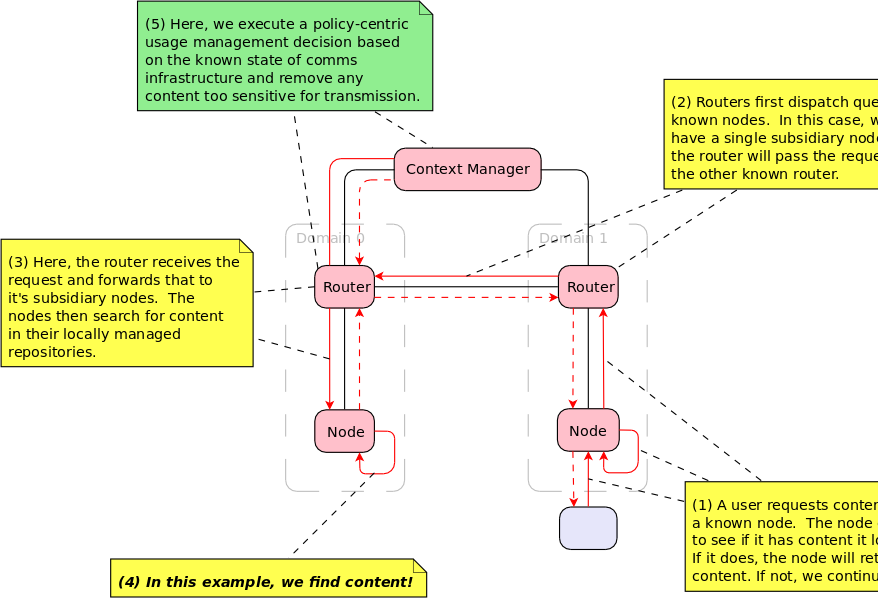
\includegraphics[width=6in]{cross-domain-prototype}
\caption{Simulation Logical Configuration}
\label{fig:model:cross-domain-prototype}
\end{figure*}

\section{Overlay Implementation Concerns}
A key concept in our current work is the separation of content management from physical communication networks.  In the past, content was controlled via partitioning and physical network access management.  Physical networks were tightly controlled as a way to manage access to sensitive content.  Classified networks in common use today are canonical examples of this kind of approach to content management.  Access to these networks is tightly controlled by classification authorities and the ability to transfer content from these networks to more open systems is rigorously managed.  Corporate systems have also commonly used this kind of approach, though not usually with so much regulation or rigor.

This kind of approach is not scalable however.  It imposes huge costs and infrastructural requirements that are becoming too large to effectively manage.  Furthermore, future systems containing sensitive information require similar security features, and simply cannot be developed without custom controlled infrastructure.  Health care systems, for example, have huge security needs and a more finely grained level of application than even deployed government systems.  These systems will contain exabytes of data, all of which needs to be explicitly controlled, managed, and reviewed by those associated with specific managed records.

Separating content networks from physical networks enables network infrastructure virtualization and multi-tenancy.  Use the popular file-sharing system BitTorrent as an example.  BitTorrent is a content network optimized for download efficiency.  It run over traditional TCP/IP networks, but manages traffic according to specialized algorithms unique to BitTorrent.  These algorithms take advantage of the asymmetry between upload and download speeds of typical home-use Internet systems in which upload speeds are regularly an order of magnitude slower than download speeds.  By partitioning content into distinct sections and downloading them from multiple clients, a downloading node can effectively use all available download bandwidth and is no longer necessarily constrained by the upload bandwidth of a serving peer system.  We use a similar approach, in that our hypothesized systems also overlay TCP/IP traffic, but rather than optimizing download speeds we focus on content usage management.

Just as systems like BitTorrent runs over current established protocols, usage management overlay systems could as well.  They support multi-tenant cloud computing systems by providing secure compartmentalized access to managed information.  They also support the ability to create and use integrated overlay systems between multiple cloud providers, supporting running of overlay components in systems hosted at Amazon while accessing nodes executing on Rackspace infrastructure.

Content networks must deal with situations analogous to those encountered in previous physical systems.  Specific examples include cross-domain monitoring and content mashing.  Both problems are currently areas of active research within physical networks and need extensive examination in overlay systems as well.

To begin with, in content-specific overlay networks, cross-domain routing can become an even more pervasive issue.  Currently, cross-domain data processing guards are installed on the perimeter of sensitive networks where they can monitor and manage outgoing and incoming traffic.  In content networks, these kinds of systems can begin to multiply within the information transmission fabric.  In physical networks, the network topology is fixed and is established when the network is installed.  After installation, changes in the essential network topology are cost-prohibitive and correspondingly rare.  Overlay systems do not suffer from this high cost of change, and can easily morph from one topology to another.  As additional content enclaves appear within a given overlay topology, the need for content usage management between those enclaves increases.

Mashup scenarios become similarly common.  As additional sources of accessible data appear, opportunities for inappropriate data combinations increase at best geometrically.  Data combinations need to be likewise managed to prevent inappropriate data combinations.

\section{Initial Prototype Implementation}
Our first completed prototype shows that overlay routers can in fact use licenses bundled alongside content to modify transmitted content based on dynamic network conditions.  Running on a single host over HTTP, it simulates two content domains and communication between them.  The communication link has uncertain security state and changes over time.  Note that this prototype currently runs on a single host with varying ports, but it could easily run on multiple hosts as well.  The current single host configuration is simply to simplify system startup and shutdown.

License bundles are hosted on the filesystem, though they could be hosted in any other data store.  These artifacts are currently XML.  They are stored in a directory, and the license file has a LIC extention while the content file has an XML extension.  Both the content and the license files have the name of the directory in which they reside (for example, if the directory is named test, the license file is named test.lic and the content file test.xml).  In this context, the directory is the content bundle.  The license and content files are simply documents and port to document-centric storage systems like MongoDB easily.  They can certainly be stored in traditional relational databases as well.

The system itself has two domains, Domain 0 and Domain 1.  Each domain consists of a client node and a content router node.  Requests are initially served to client nodes.  If client nodes do not contain the requested content, they the forward that request to their affiliated content router.  The content router will send that request to all the content routers of which it is aware.  Those other routers will then query associated client nodes for content.  If the requested content is in fact found, it will be returned to the original requesting router and then to the requesting node.  If the content is not found, HTTP status 404 codes are returned to requesting routers and nodes.

All router-to-router content traffic is modified based on security conditions.  A Context Manager maintains metadata regarding network paths.  If a given network path is only cleared for data of a certain sensitivity level, a transmitting router will remove all license information and content that is associated with higher sensitivities, and then transmit only information at an appropriate sensitivity level over the link.

Figure \ref{fig:model:cross-domain-prototype} shows the prototypical workflow through the system across the domains, and Figure \ref{fig:model:prototype-physical-config} shows the current system configuration of the simulation, with the cross-domain link highlighted in red.  The system is current configured to use ports 4567 through 4571.

All content requests are via HTTP GET.  Link status can be changed via HTTP POST and we use the CURL command to exercise the network.

This proof-of-concept does implement a simple overlay network for usage managed content over HTTP, easily extensible to HTTPS.  Changes in the context of the network dynamically change the format of transmitted content.  All source code for this simulation is publically available on GitHub, at https://github.com/cclamb/overlay-network, with documentation on how to run the simulation.

\begin{figure}[!t]
\centering
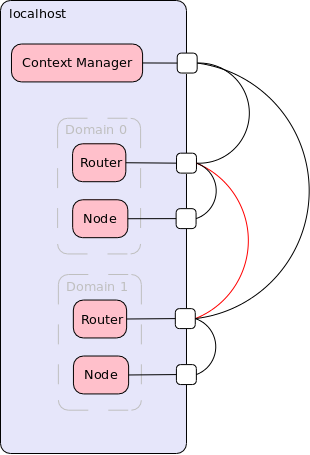
\includegraphics[width=3in]{prototype-physical-config}
\caption{Physical Simulation Configuration}
\label{fig:model:prototype-physical-config}
\end{figure}

\section{Initial Prototype Results}

Policy and content delivery over HTTP possible

Ruby/Sinatra will support HTTP overlay development, CURL for usage

Information Filtering Expectations

Extension into larger distributed system feasible

\section{Inter-Provider Cloud Configuration}
Over the month of June we established our initial technical baseline for upcoming content network development.  We have created and deployed baseline system images in both Amazon's Elastic Compute Cloud (EC2) and Rackspace Servers infrastructures.  We have also created and exercised our deployment, configuration, and logging systems to enable distributed monitoring and centralized reporting.  Overall, we currently have 20 nodes running with two distinct providers geographically dispersed across the continental United States.  This leads to a distinct requirement for a centralized system with distributed access for both initial configuration information as well as logging and auditing.  We have implemented this required infrastructure using Amazon's Simple Storage Service (S3), accessible from both Rackspace and Amazon hosted virtual machines.
The specific technical components are Amazon EC2, Amazon S2, Rackspace Servers, and GitHub.  Both EC2 and Rackspace nodes are Ubuntu virtual machines, albeit at different versions, as we run Ubuntu version 11.04 in Rackspace and Ubuntu Version 12.04 in Amazon's infrastructures.  These systems are provisioned with Git, Ruby, the Ruby Version Manager (RVM), and supporting libraries.  They all run as micro-intances or equivalent, and are bootstrapped with the appopriate project information to begin to participate as an overlay network node.  While EC2 and Rackspace Server infrastructures are infrastructure-as-a-cloud (IaaS) offerings supporting virtual machine instances of various types, Amazon S3 is a simple key-value store.  Running with REST sematics over HTTP, S3 stores arbitrary documents associated with specific keys in buckets.  These documents can be downloaded by any authorized participant, where authoriztion state is proven by possention of a secret key.  In this way, we can store the global configuration of a specific overlay network in a single location from which every node can access informationm with respect to their pending role and needed configuraiton information.  Likewise, all overlay network state can also be saved to centralized buckets for later analysis.  Finally, Github is a centralized source code repository used to share code between all participating nodes.  Prior to each content network instantiation, each node checks the repository for updates, and downloads them if they exist.

All data saved within S3 is serialized in a text-based data serialization language known as YAML.  YAML is a widely supported hierarchical data representation language with support within the Ruby core platform.  This enables us easily serialize Ruby-native data structures to text-based representations for storage within S3.  More importantly, it simplifies post-experimental data analysis as any information logged to the centralized logging system during a given experimental run can be easily read and analyzed after the fact.

In order to manage and initialize all overlay nodes, we use Capistrano.  Capistrano is a distributed deployment system initially used to manage large clusters of Ruby-on-Rails systems.  It has since expanded into a general-purpose distributed deployment toolchain, tightly integratd with Git.  This allows us to bootstrap different configurations of networks from a single command-and-control node simply and efficiently.

\begin{table*}[tp] %
\centering %
\begin{tabular}{clcc}
\toprule %
$Category$ 				& $Components$ 								\\\toprule %
$Infrastructure$ 		& Amazon S3, Amazon EC2, Rackspace Servers 	\\\midrule
$Operating Systems$		& Ubuntu 11.04, Ubuntu 12.04 				\\\midrule
$Technologies$			& Ruby (Sinatra, Capistrano, YAML) 			\\\midrule
$Supporting Systems$	& Git, Github 								\\\bottomrule
\end{tabular}
\caption{Supporting Components}
\label{table:model:components}
\end{table*}

All these infrastructural elements, protocols, and technology components have been successfully tested, allowing for unified control and configuration of large, distributed overlay systems.  We have successfully tested our logging systems, and integrated them with the Ruby runtime for ease of access.  We have also passed configuration information to both Rackspace and Amazon EC2 systems and verified access from all participating nodes.  Finally, we have successfully exercised the ability to dynamically update all participating nodes from Github as well as the capability to manage the system via Capistrano.

